\chapter{Ruby on Rails y patrones Web 2.0} % (fold)
\label{cha:ruby_on_rails_y_patrones_web_2_0}

  \section{Porque usar Ruby on Rails para desarrollar una aplicación web ?} % (fold)
  \label{sec:porque_usar_ruby_on_rails_para_desarrollar_una_aplicacion_web}

    La gran propaganda de Ruby on Rails (RoR) o más sencillamente Rails
    se basa en el rápido desarrollo de aplicaciones web, conocido como agile development.
    Como parte de su construcci\'on, Rails maneja las filosofías \emph{DRY}\footnote{Don’t Repeat Yourself} y \emph{convención sobre configuración}. 

    \begin{description}
      \item[No te repitas(DRY)] según el creador de RoR, \mbox{David} \mbox{Heinemeier} Hansson, 
      significa que cada pieza de conocimiento en un sistema 
      debe ser declarado en un solo lugar.\cite{awdr4e} 
      Esto lo logra gracias al patrón Modelo-Vista-Controlador\footnote{MVC}, 
      y el lenguaje multiparadigma Ruby sobre el cual está construido Ruby on Rails.
      
      \item[Convención sobre configuración] significa que Rails tiene parámetros por 
      defecto para casi todos los aspectos que mantiene unida una aplicación, ya que se logro
      observar que la gran mayoria de aplicaciones web compartian la misma configuracion inicial,
      siguiendo  las convenciones de Rails se llega a simplificar el código escrito en una aplicación.
    \end{description}


    David Heinemeier cita en su libro \cite{awdr4e}, que \emph{“Rails es Ágil porque 
    simplemente la agilidad es parte de su construcción”}.

    Se puede analizar esta afirmaci\'on teniendo en cuenta los principios del
     \textbf{manifiesto por el desarrollo ágil de software}\footnote{http://agilemanifesto.org/iso/es/}:
    \begin{itemize}
      \item \textbf{Individuos e interacciones} sobre procesos y herramientas
      \item \textbf{Software funcionando} sobre documentación extensiva
      \item \textbf{Colaboración con el cliente} sobre negociación contractual
      \item \textbf{Respuesta ante el cambio} sobre seguir un plan
    \end{itemize}
    
    Rails se enfoca bastante en conseguir un prototipo funcional en muy poco tiempo 
    y sobre ese prototipo seguir incrementalmente hasta conseguir una aplicacion 
    de calidad.\\
     % en poco tiempo.\\

    Los más grandes obstáculos que se enfrenta una aplicación en el tiempo es el 
    mantenimiento y escalabilidad, actualmente se estima que existen 230,000 websites\cite{web2} 
    desarrolladas sobre RoR %\footnote{Ruby on Rails, tambien se lo puede nombrar \emph{Rails}, \emph{RoR}}, 
    entre ellas se puede nombrar a GitHub, Hulu, Yellow Pages. Son sitios con miles de visitas diarias
    con una alta carga del servidor y son un claro ejemplo de que Rails puede manejar sitios de alto perfil.\\

    Los detractores de Rails sostienen que escalar una aplicación construida 
    sobre RoR es muy difícil pero los defensores argumentan que lo que se 
    tiene que escalar es el código de la aplicación no el framework.\\

    Twitter nació sobre Ruby on  Rails  y no fue hasta que era un servicio usado 
    a nivel mundial y manejaba millones de request por día que empezaron a surgir 
    problemas debido a que Ruby no estaba optimizado para un trabajo muy pesado, 
    según palabras de Alex Payne, Twitter developer, “Ruby es lento”\cite{web3}. 
    Actualmente Twitter migró su backend a Scala, framework basado en Java(que esta mas optimizado que Ruby),
    pero para su front-end no cambian a Rails.\cite{web4}\\
    
    Se puede agregar que Rails es una muy buena opción a la hora de empezar 
    cualquier proyecto web, ya que implementa las herramientas necesarias 
    para un desarrollo ágil, sólido y de calidad respaldado por un modelo 
    de desarrollo basado en pruebas(TDD\footnote{Test Driven Development}), las filosofías DRY y convención sobre configuración.
    y cundo la aplicaci\'on haya crecido y empiecen a aparecer los problemas es 
    decisión de los programadores el ver si mantener el código actual y parchearlo o 
    cambiar de tecnología para mejorar el rendimiento y la experiencia del usuario\\
  % section porque_usar_ruby_on_rails_para_desarrollar_una_aplicacion_web (end)

  \section{Patrones de diseño de la Web2.0} % (fold)
  \label{sec:patrones_web20}
    Que es la Web2.0 ?,  primeramente  se debe explicar que este término fue acuñado 
    por 1999 para describir paginas web que usaban tecnologias mas alla de las 
    simples estaticas paginas web.
    
    No fue hasta que en  el 2004 en la conferencian sobre la Web2.0 que se popularizo este termino, 
    y asi mismo como la Web que evoluciona, la definicion se actualiza con el tiempo, 
    y Tim O’Reilly trato de definirla en su articulo ``\emph{What is Web 2.0}''\cite{web5},
    articulo que se puede considerar como la guia de referencia para cualquier persona que quiera
    entender que es la Web2.0 y sus origenes,
    en un articulo posterior ``\emph{Web 2.0 Compact Definition: Trying Again}''\cite{web9}
    del que se puede extraer la siguiente definici\'on:
    \begin{quote}
      “Web 2.0 is the business revolution in the computer industry caused by the move to the
       Internet as a platform, and an attempt to understand the rules for success on that new
       platform. Chief among those rules is this: build applications that harness network
       effects to get better the more people use them.”
       \begin{flushright}
       --Tim O’Reilly
       \end{flushright}
    \end{quote}
    En resumen se puede definir que una aplicación web2.0 es aquella que mejora y crece con la 
    participación activa de sus usuarios.

    \begin{quote}
      “Software que mejora mientras más gente la usa” \cite{web5}
    \end{quote}

    Un patrón de diseño es una solución general, reusable  y flexible 
    que describe cómo resolver algún problema general en el desarrollo 
    de software, un patrón puede ser usado y modificado segun el problema 
    al cual se esta aplicando.\\
    Se pueden observar los siguientes patrones de dise\~no en la aplicación:
    \begin{itemize}
      \item \textbf{REST}
      \item \textbf{MVC}
      \item \textbf{Mashup}
    \end{itemize}

    \subsection{REpresentational State Transfer (REST)} % (fold)
    \label{sub:rest}
      REST es un término descrito por Roy Fielding en su tesis doctoral ``\emph{Architectural Styles and the design of Network-based Software Architectures}''\cite{web6}, describe estilos arquitectónicos de sistemas interconectados por red.

      REST es un estilo arquitectónico que especifica cómo los recursos van a ser definidos y direccionados, especifica la importancia del protocolo \emph{cliente-servidor-sin estado}, ya que cada request tiene toda la información necesaria para entenderla.\\

      En el contexto de Rails, REST significa que los componentes del sistema por ejemplo los usuarios son modelados como recursos que pueden ser creados, leidos, actualizados y borrados, estas acciones corresponden a las operaciones CRUD (Create, Read, Update, Delete) de las base de datos relacionales  y a los cuatro operaciones fundamentales POST, GET, PUT, DELETE definidos en el  protocolo HTTP.\\

      En Rails el estilo de desarrollo RESTful\footnote{se denomina RESTful a los sistemas que siguen los principios REST} ayuda a determinar acerca de qué controlador y cuál será la acción que se ejecutará, solamente procesando el request HTTP hecho al servidor.\\

      \textbf{GET} es la operación HTTP más común, es usado para leer datos en este caso paginas, se puede leer como ``get a page'', \textbf{POST} es la operación que se usa cuando se ejecuta un formulario, en la convención de Rails \textbf{POST} se usa para crear objetos o recursos, PUT se usa para actualizar objetos ,DELETE se usa para borrar objetos.  Los browsers actuales no son capaces de manejar las operaciones \textbf{PUT} y \textbf{DELETE} de forma nativa, por lo que Rails usa un pequeño truco que consiste en declarar el método que se esta enviando en un \emph{hidden field} en el formulario HTML.\\

      Para lograr todo este comportamiento  es necesario declarar, en el archivo que controla las rutas dentro de la aplicación, \textbf{routes.rb}, que el recurso usuarios es \emph{restful}, tal como se muestra en la figura \ref{fig:rest}\\

      \begin{figure}[!hbp]
        \begin{center}
          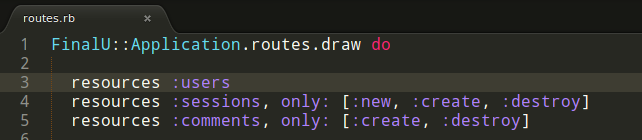
\includegraphics[width=1\textwidth]{rest}
        \end{center}
        \caption[REST - routes.rb]{config/routes.rb}
        \label{fig:rest}
      \end{figure}

      La imagen \ref{fig:rest} muestra como se declara a \textbf{users} con 
      todas las acciones restful los cuales se listan en el cuadro \ref{tab:rest},  
      Rails también permite declarar solamente algunas acciones restful,
      como se ve el recurso \textbf{sessions} solamente tiene las acciones de \textbf{new}, \textbf{create} y \textbf{destroy}.\\
     

      \begin{table}[!hbp]
        \label{tab:rest}
        \begin{center}
          \begin{tabular}{ lll }
            \multicolumn{1}{c}{\textbf{HTTP request}} & \multicolumn{1}{c}{\textbf{URL}}  & \multicolumn{1}{c}{\textbf{ACTION}} \\
            \toprule
            GET     &   /users         &   index \\ %\hline
            GET     &   /users/1       &   show \\
            GET     &   /users/new     &   new \\
            POST    &   /users         &   create \\
            GET     &   /users/1/edit  &   edit \\
            PUT     &   /users/1       &   update \\
            DELETE  &   /users/1       &   destroy \\
            \bottomrule
          \end{tabular}
          \caption[recursos REST]{las posibles rutas que se generan}
        \end{center}
      \end{table}

      Por ejemplo, si generamos una petición GET hacia la direccion  \emph{/usuarios/1} el servidor interpreta la dirección y responde mostrando la información del usuario “1” ejecutando la acción \textbf{show} del controlador usuarios y en cambio si se genera una petición PUT a la misma direccion \emph{/usuarios/1} el servidor procesa la información y ejecuta la acción \textbf{update} del controlador usuarios actualizando la información del usuario “1”. Estas acciones no son más que métodos dentro del \emph{user\_controller.rb} el cual es parte del controlador de la arquitectura MVC.\\

      Esta convención de Rails ayuda a entender de mejor manera el flujo que tiene un recurso, 
      las URL son legibles y únicos para cada recurso. La implementación de los recursos se hace mas limpia y ordenada situaciones que son claves para el mantenimiento y la extensibilidad del sistema.
    % subsection rest (end)

    \subsection{MVC} % (fold)
    \label{sub:mvc}
      MVC (Modelo Vista  Controlador) es un patrón arquitectónico que separa los datos de la aplicación en la interfaz del usuario y  la lógica del negocio en tres partes cada uno especializado para su tarea, la vista maneja lo que es la interfaz del usuario puede ser gráficamente o solo texto, el controlador interpreta las entradas del teclado, mouse, o los cambios de la vista de la mejor forma y finalmente el modelo maneja el comportamiento de los datos de la aplicación.\cite{web7}\\

      Concepto que se desarrolló en 1979 por Trygve Reenskaug el cual da una solución al problema de separar la lógica del negocio de la lógica de la presentación. Cada acción o concepto se desarrolla en un lugar determinado, los objetivos que se pueden apreciar al usar esta arquitectura es la facilidad para escribir código y de mantenerlo. \\

      Se puede apreciar el comportamiento de este patrón, en la figura \ref{fig:mvc}, al visitar la ruta que muestra la información de un usuario ``\emph{localhost/users/1}'' desde el navegador, este genera una llamada GET y Rails lo direcciona a la acción show del \textbf{controlador} users, la acción show se encarga de llamar al \textbf{modelo} “User”, el controlador extrae el id del usuario de la llamada\footnote{request} \textbf{ GET /users/1 }, permitiendo al \textbf{modelo} que es el encargado de manejar la lógica del negocio, por ejemplo validando o modificando los datos que se guardan o se extraen de una base de datos, el controlador almacena la información devuelta por el modelo en la variable @user, que es pasada a la \textbf{vista} show.html.erb el cual se encarga de generar el template HTML y devuelve al navegador la página solicitada. \\

      La capacidad de declarar una variable en el controlador y que esta variable esté disponible en la vista, así como toda la configuración que envuelve el comportamiento del patrón MVC ya esta implementada y no es necesario crear archivos de configuración, todo este trabajo es parte de la filosofía de Rails “convención sobre configuración”.\\

      \begin{figure}[!hbp]
        \begin{center}
          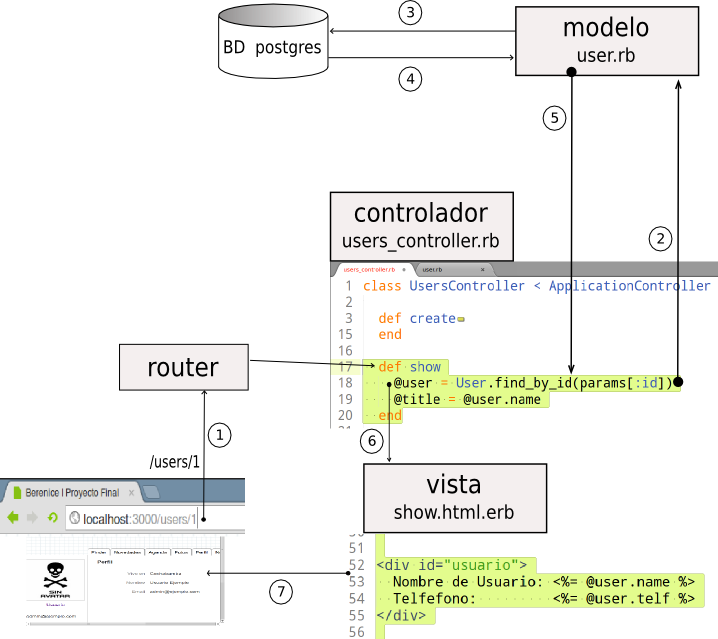
\includegraphics[width=1\textwidth]{mvc}
        \end{center}
        \caption{Un diagrama detallado del patr\'on MVC en Rails}
        \label{fig:mvc}
      \end{figure}
    % subsection mvc (end)

    \subsection{Mashup} % (fold)
    \label{sub:mashup}
      Mashup es una técnica en el desarrollo de aplicaciones web que consiste en combinar datos de diferentes proveedores. Un mashup usa uno o más servicios y mezcla algunas características de estos servicios, los servicios generalmente son datos que son distribuidos mediante las APIs\footnote{Application Programming Interface, es el conjunto de funciones y procedimientos que se ofrece para ser utilizado por otro software}. Con la finalidad de ofrecer estos datos de forma más fácil de entender y usar para el cliente.\\

      Los primeros mashups empezaron como experimentos con los web services que ofrecian las grandes empresas, por ejemplo uno de los primeros mashups importante fue el de housingmaps.com  que convina los datos de Craigslist ( listas de casas, departamentos, etc, para rentar, vender ) y Google Maps ( mapas a nivel global), en una aplicaci\'on que ofrece servicios y los se\~nala en un mapa. Desde entonces surgieron diferentes tipos y aproximaciones dependiendo del tipo de datos y el servicio que se quiere ofrecer.\cite{web8}\\

      Se pueden apreciar diferentes implementaciones de mashups, los mashups orientados al consumo y los mashups orientados a las empresas, básicamente estos mashups de consumo se refieren a aplicaciones en las cuales los datos obtenidos de diferentes fuentes son mezclados y presentados al cliente, y los mashups empresariales o de negocios aparte de las fuentes de datos externas, mezclan sus propios datos en el mashup ofreciendo una mejor experiencia del usuario.\\

      Uno de los componentes básicos de la Web 2.0 son los \textbf{datos}, sobre los cuales se puede obtener un producto con valor agregado, los datos están disponibles para que sean usados, pero obtener y almacenar estos ``datos''  y dependiendo del tipo de datos, puede llegar a costar tiempo o dinero o ambos, es por eso que los datos son ofrecidos con o sin restricción dependiendo de las políticas de uso que tenga la empresa que ofrece los datos.\\

      En la aplicación desarrollada se necesitaba el uso de mapas para que el despliegue de información sea de forma más interactiva y de fácil uso, los datos geográficos públicos generalmente están disponibles para ser usados pero para su uso se necesitaba que esté representado de forma gráfica en la pantalla de la computadora, este trabajo lo llevan a cabo empresas las cuales generalmente cobran por el uso de los mapas, se puede  apreciar que se están obteniendo datos en forma de mapas a través del API de Google Maps, Google permite usar sus datos con restricciones dependiendo de la cantidad de llamadas que se haga a su API por la aplicación que la usa.\\

      El gran beneficio de usar los datos de Google Maps en un mashup es que nos permite desplegar información que de otra forma costaría mucho tiempo y dinero para implementar.\\

      Para usar el API de Google Maps solo es necesario importar la librería declarandola en la cabecera del documento HTML, para visualizar el mapa es necesario declarar un elemento único (se recomienda un div con id de preferencia ``map'' o similares) dentro del DOM de la página y se maneja mediante el lenguaje de programación del lado del cliente: javascript.\\

      \begin{figure}[!hbp]
        \begin{center}
          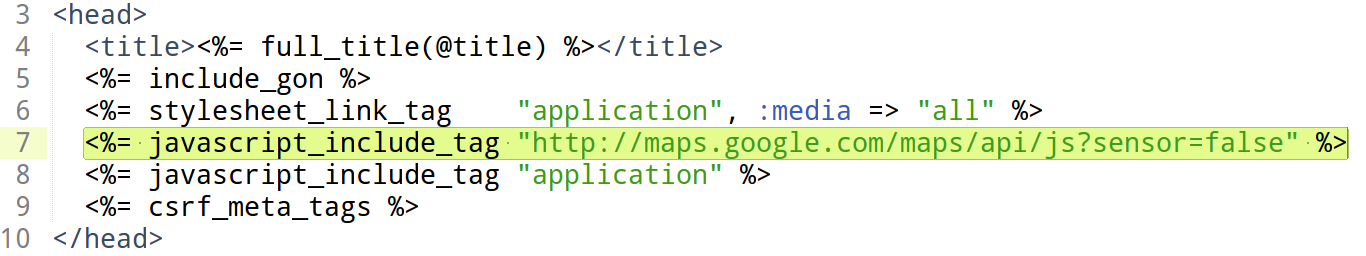
\includegraphics[width=1\textwidth]{api_gms}
        \end{center}
        \caption[API de Google Maps declarado]{Se importa el API de Google Maps declarando en  <head>  ~del documento}
        \label{fig:api_gm}

      %   \hspace{4em}

      %   \begin{center}
      %     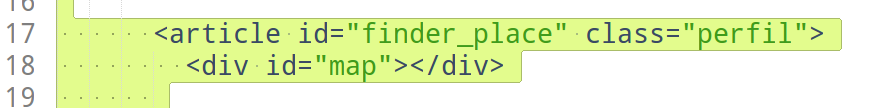
\includegraphics[width=1\textwidth]{div_map}
      %   \end{center}
      %   \caption[Div con id map para el Mapa]{El mapa se visualiza dentro de la etiqueta div con id map}
      %   \label{fig:div_map}

      %   \hspace{4em}

      %   \begin{center}
      %     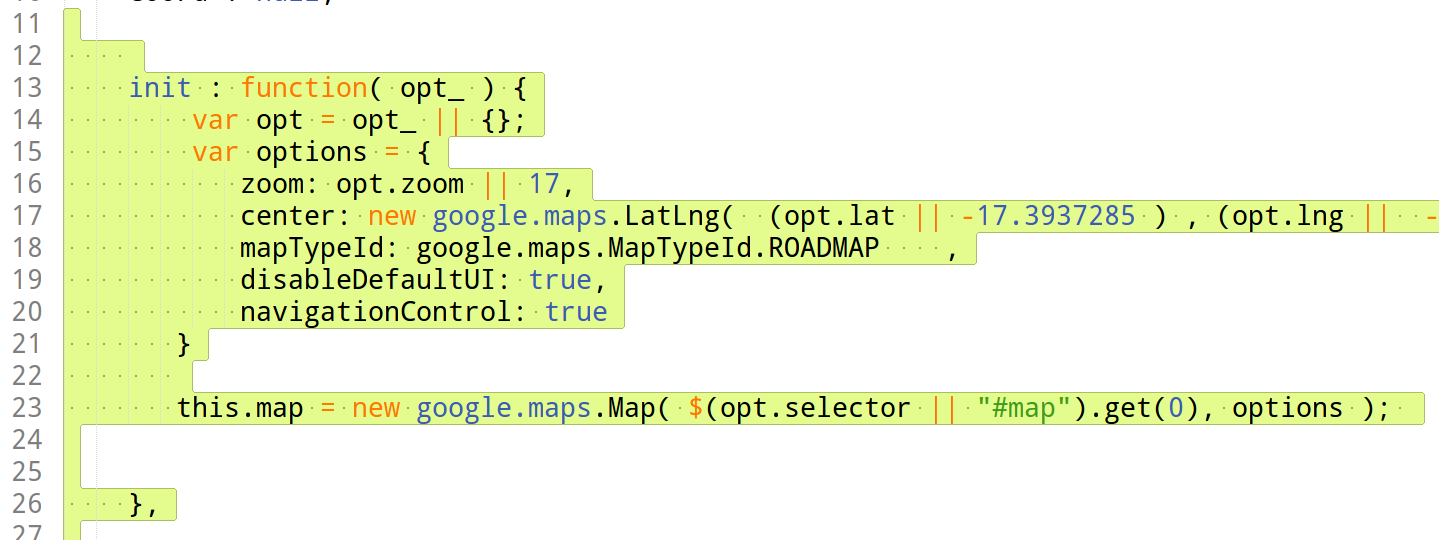
\includegraphics[width=1\textwidth]{umss_init}
      %   \end{center}
      %   \caption[UMSS javascript]{Se captura el div map del documento y se inicializa el mapa mediante el lenguaje javascript}
      %   \label{fig:umss_js}
      \end{figure}
      
        % \vspace{4em}
      \begin{figure}[!hbp]
        \begin{center}
          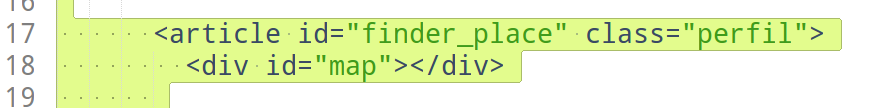
\includegraphics[width=1\textwidth]{div_map}
        \end{center}
        \caption[Div con id map para el Mapa]{El mapa se visualiza dentro de la etiqueta div con id map}
        \label{fig:div_map}
      \end{figure}


      \begin{figure}[!hbp]
        \begin{center}
          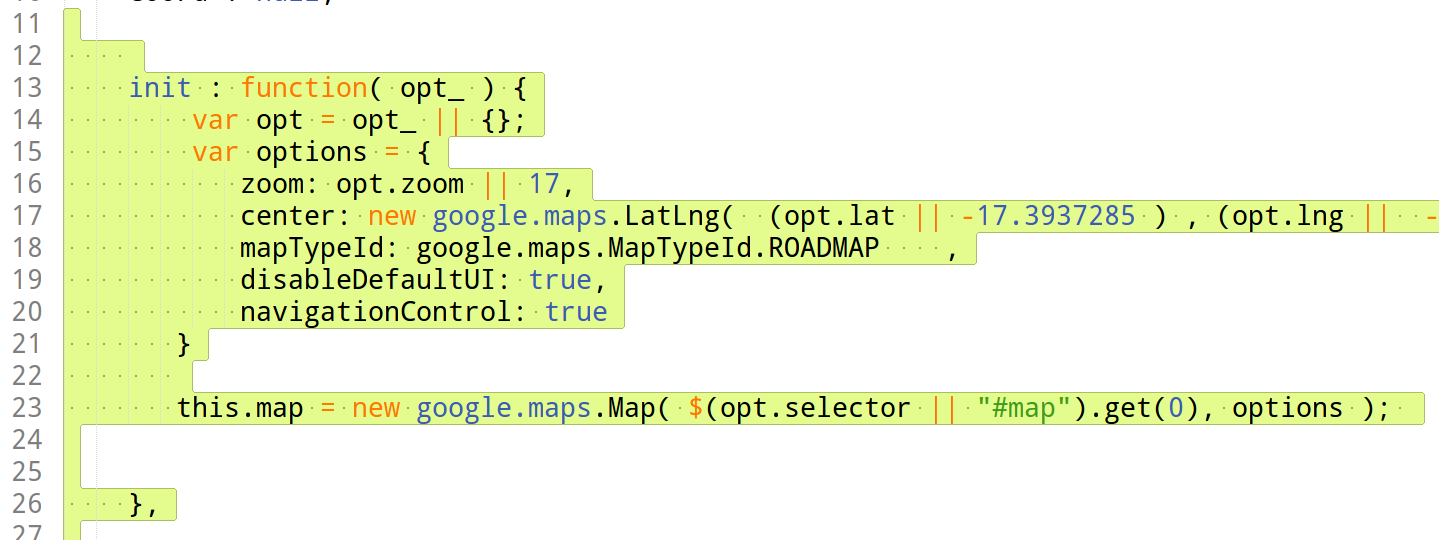
\includegraphics[width=1\textwidth]{umss_init}
        \end{center}
        \caption[UMSS javascript]{Se captura el div map del documento y se inicializa el mapa mediante el lenguaje javascript}
        \label{fig:umss_js}
      \end{figure}

    % subsection mashup (end)
  % section patrones_web20 (end)
% chapter ruby_on_rails_y_patrones_web_2_0 (end)


